\documentclass[
  aspectratio=1610,
]{beamer}

% chktex-file 1
% chktex-file 26

\usefonttheme{professionalfonts}
\usefonttheme[stillsansseriflarge, stillsansserifsmall]{serif}

%\usetheme{Frankfurt}
%\usecolortheme{dove}

\usepackage{amsmath, amssymb}
\usepackage{booktabs}

\usepackage[MnSymbol]{mathspec}
\defaultfontfeatures{
  Ligatures=TeX,
  Scale=MatchLowercase,
}
\setsansfont{Gill Sans}
\setmainfont{Minion Pro}
\setmonofont{Fira Mono}

\usepackage{xltxtra}
\usepackage{polyglossia}
\setdefaultlanguage{german}

\usepackage{hyperref}

\usepackage{minted}

\setbeamertemplate{navigation symbols}{}

\graphicspath{{./bilder/}}

\newcommand{\wplogo}{
\includegraphics[height=2ex]{enwiki.png}}

\author{Martin Darmüntzel}
\title{Einführung in C}
%\subtitle{}
\institute{Universität Rostock}
%\date{6. September 2019}

\begin{document}

\begin{frame}
  \titlepage{}
\end{frame}

% \section{Geschichte}%

\begin{frame}
  \begin{center}
    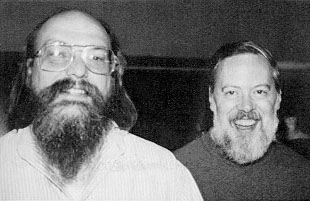
\includegraphics{Ken_Thompson_and_Dennis_Ritchie--1973.jpg}

    Ken Thompson \& Dennis Ritchie
  \end{center}
  \tiny Quelle:
  \url{https://en.wikipedia.org/wiki/File:Ken_Thompson_and_Dennis_Ritchie--1973.jpg}
\end{frame}

\begin{frame}
  \begin{center}
    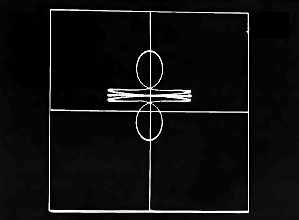
\includegraphics{Space_Travel_Screenshot.png}

    Space Travel
  \end{center}
  \tiny Quelle:
  \url{https://en.wikipedia.org/wiki/File:Space_Travel_Screenshot.png}
\end{frame}

\begin{frame}
  \begin{center}
    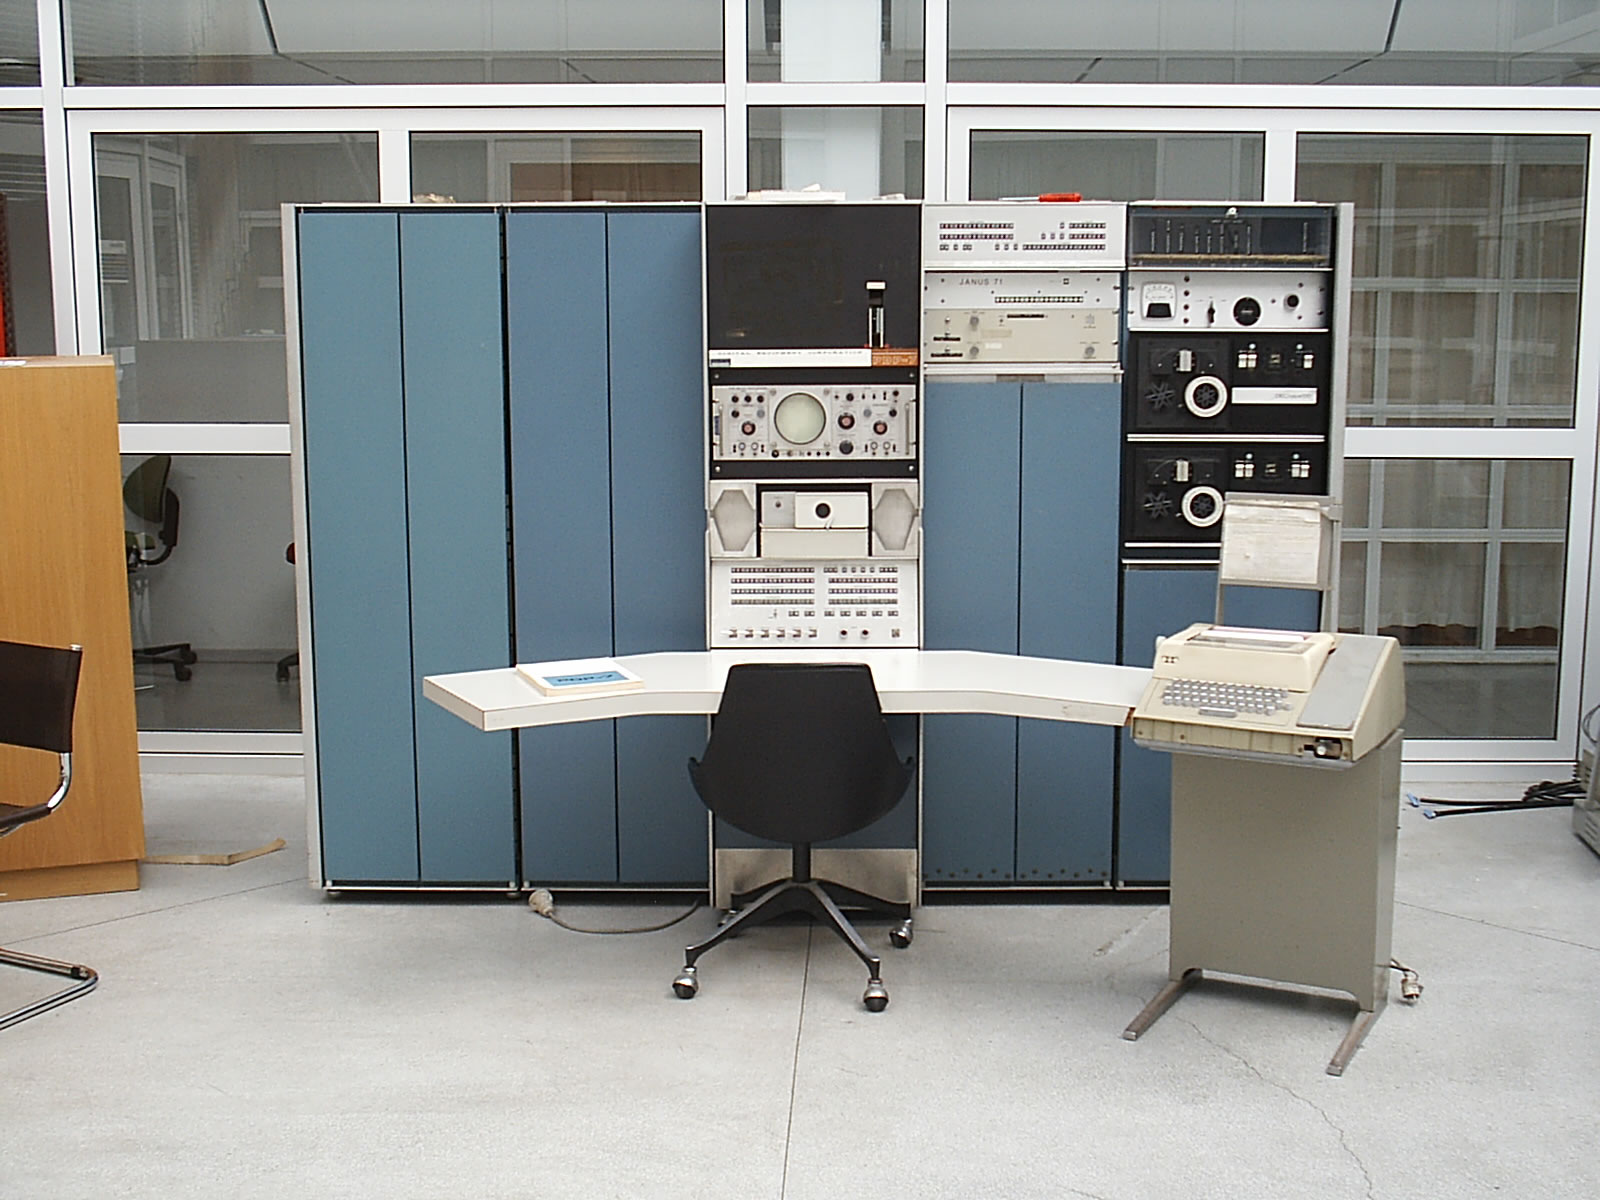
\includegraphics[width=0.75\textwidth]{Pdp7-oslo-2005.jpeg}

    PDP-7
  \end{center}
  \tiny Quelle:
  \url{https://upload.wikimedia.org/wikipedia/commons/5/52/Pdp7-oslo-2005.jpeg}
\end{frame}

\begin{frame}{Programmierprobleme unserer Großeltern}
  \begin{itemize}
    \item viele verschiedene Computer- bzw. Prozessorhersteller
    \item viele verschiedene Architekturen mit verschiedenen Instruktionssätzen

      siehe z.\,B.
      \href{https://en.wikipedia.org/wiki/Comparison_of_instruction_set_architectures}{Comparison
      of instruction set architectures \wplogo}
    \item viele verschiedene Maschinensprachen bzw. Assemblersprachen
    \item[$\rightarrow$] ein Programm für einen PDP-7 lief nicht auf einem Intel-Prozessor
  \end{itemize}

  \pause{}
  \vspace{1em}

  Lösung: Abstraktion durch Hochsprachen

  \begin{itemize}
    \item Fortran (1957)
    \item ALGOL (1958)
    \item LISP (1958)
    \item[$\rightarrow$] C (1972)
  \end{itemize}
\end{frame}

\begin{frame}{Warum C?}
  \begin{itemize}
    \item simple Syntax
    \item flexibel und portierbar
    \item abstrakt genug $\leftrightarrow$ konkret genug („Hochsprachen-Assembler“)
    \item Grundlage für viele wichtige Programme und andere Programmiersprachen
  \end{itemize}
\end{frame}

\begin{frame}{Programmieren im Allgemeinen}
  Mensch schreibt Quelltext
  $\rightarrow$ Compiler produziert Programm aus Maschinencode
  $\rightarrow$ Betriebssystem führt Programm aus

  \pause{}

  \begin{block}{Wichtig}
    Quelltext wird für Menschen geschrieben, nicht für Maschinen!
  \end{block}
\end{frame}

\begin{frame}{Handwerkszeug}
  \begin{itemize}
    \item Quelltext schreiben: Texteditor,
      z.\,B. \texttt{gedit}, \texttt{vim}, \texttt{emacs}
    \item Compiler: \texttt{gcc}, \texttt{clang}, meist einfach nur \texttt{cc}
    \item Programm ausführen: Terminal
  \end{itemize}

  \pause{}

  \begin{block}{Wichtige Basisbefehle im Terminal}
    \begin{description}
      \item[\texttt{pwd}] zeigt das aktuelle Verzeichnis an
      \item[\texttt{ls}] listet den Verzeichnisinhalt auf
      \item[\texttt{cd}] wechselt das Verzeichnis
        \begin{itemize}
          \item \texttt{cd ..} wechselt in das übergeordnete Verzeichnis % chktex
        \end{itemize}
      \item[\texttt{cc}] kompiliert Quelltext
        \begin{itemize}
          \item \texttt{\$ cc hello.c} erzeugt die ausführbare Datei \texttt{a.out}
          \item \texttt{\$ ./a.out} führt sie aus
          \item \texttt{\$ cc -o hello hello.c} erzeugt die ausführbare Datei \texttt{hello}
          \item \texttt{\$ ./hello} führt sie aus
        \end{itemize}
    \end{description}
    Bitte abschreiben!
  \end{block}
\end{frame}

\begin{frame}{Hello, world!}
  \inputminted{c}{hello.c}

  \pause

  \begin{block}{Aufgabe}
    Öffne einen Texteditor (z.\,B. \texttt{gedit}), schreibe den Quelltext ab und
    speichere ihn in der Datei \texttt{hello.c}.

    Öffne ein Terminal und kompiliere die Datei mittels \texttt{cc hello.c}.

    Führe das erzeugte Programm mittels \texttt{./a.out} aus.
  \end{block}
\end{frame}

\begin{frame}{Rechnen}
  \inputminted{c}{rechnen.c}

  \begin{columns}[T]
    \begin{column}{0.3\textwidth}
      \begin{tabular}{lc}
        \toprule
        Rechenart & Operator\\
        \midrule
        Addition       & \texttt{+}\\
        Subtraktion    & \texttt{-}\\
        Multiplikation & \texttt{*}\\
        Division       & \texttt{/}\\
        Modulo         & \texttt{\%}\\
        \bottomrule
      \end{tabular}
    \end{column}
    \begin{column}{0.5\textwidth}
      \pause

      \begin{block}{Aufgabe}
        Schreibe das Programm ab und überprüfe die Ausgabe.\\[1ex]

        Schreibe ein Programm, das für alle Zahlen von \texttt{1} bis \texttt{6} das
        Ergebnis der Berechnungen \texttt{6/1}, \texttt{6/2}, \ldots\ und \texttt{6\%1},
        \texttt{6\%2}, \ldots\ ausgibt.
      \end{block}
    \end{column}
  \end{columns}
\end{frame}

\begin{frame}{Variablen}
  \begin{itemize}
    \item wesentliches Element der Programmierung: Speichern von Daten
    \item Daten bestehen nur aus Einsen und Nullen
    \item Variable deklarieren = Speicherplatz reservieren
    \item Variable besteht aus \emph{Bezeichner} und \emph{Typ} (Ganzzahl, Gleitkommazahl,
      Buchstabe, \ldots)
  \end{itemize}
  \pause{}
  \inputminted{c}{variablen1.c}
\end{frame}

\begin{frame}{Typen}
  \begin{center}
    \begin{tabular}{ll}
      \toprule
      \texttt{char} & Zeichen oder ganzzahliger Wert\\
      \texttt{short int} & ganzzahliger Wert\\
      \texttt{int} & ganzzahliger Wert\\
      \texttt{long int} & ganzzahliger Wert\\
      \texttt{long long int} & ganzzahliger Wert\\
      \texttt{float} & Fließkommazahl (einfache Genauigkeit)\\
      \texttt{double} & Fließkommazahl (doppelte Genauigkeit)\\
      \texttt{long double} & Fließkommazahl (zusätzliche Genauigkeit)\\
      \bottomrule
    \end{tabular}
  \end{center}
\end{frame}

\begin{frame}{Ausgabe}
  \begin{itemize}
    \item \texttt{printf(} % chktex 9 chktex 36
      \textit{Zeichenkette mit Platzhaltern}
      \texttt{,}
      \textit{Argumente \ldots}
      \texttt{)}\\[2ex] % chktex 9

      \begin{tabular}{ll}
        \toprule
        Platzhalter & Typ\\
        \midrule
        \texttt{\%c} & \texttt{char}\\
        \texttt{\%i} & \texttt{int}\\
        \texttt{\%li} & \texttt{long int}\\
        \texttt{\%u} & \texttt{unsigned int}\\
        \texttt{\%lu} & \texttt{unsigned long int}\\
        \texttt{\%f} & \texttt{float}\\
        \texttt{\%lf} & \texttt{double}\\
        \texttt{\%Lf} & \texttt{long double}\\
        \bottomrule
      \end{tabular}
  \end{itemize}
\end{frame}

\begin{frame}{Eingabe}
  \begin{itemize}
    \item \texttt{scanf(} % chktex 9 chktex 36
      \textit{Zeichenkette mit Platzhaltern}
      \texttt{,}
      \textit{(Adressen von) Argumenten \ldots}
      \texttt{)} % chktex 9

      \pause{}

      \inputminted{c}{eingabe.c}
  \end{itemize}

  \pause

  \begin{block}{Aufgabe}
    Ändere das Programm so ab, dass es das nächsthöhere \emph{runde} Alter und die
    verbleibenden Jahre dahin ausgibt. Beispiel:

    \inputminted{text}{eingabe_beispiel.txt}
  \end{block}

\end{frame}

\begin{frame}{Werte zuweisen}
  \begin{columns}[T]
    \begin{column}{0.40\textwidth}
      \inputminted{c}{zuweisung.c}
    \end{column}
    \begin{column}{0.60\textwidth}
      \begin{itemize}
        \item \texttt{=} ist in C der \textbf{Zuweisungsoperator}.
        \item \textit{Variable} \texttt{=} \textit{Ausdruck}\texttt{;}
        \item rechte Seite wird ausgewertet und erst dann der Variable zugewiesen
      \end{itemize}

      \pause

      \begin{block}{Aufgabe}
        Schreibe ein Programm, das vom Nutzer den Radius eines Kreises erfragt und daraus
        den Umfang und Flächeninhalt berechnet und ausgibt. Welchen Typ muss der Radius
        haben?
      \end{block}
    \end{column}
  \end{columns}
\end{frame}

\begin{frame}{Bedingte Ausführung}
  \begin{columns}[T]
    \begin{column}{0.45\textwidth}
      \inputminted[tabsize=4]{c}{bedingung.c}
    \end{column}
    \begin{column}{0.45\textwidth}
      \pause

      \begin{itemize}
        \item \texttt{if (} % chktex 9
          \textit{Bedingung}
          \texttt{) \{} % chktex 9

          \quad\textit{Anweisungen bei wahrer Bed.}

          \texttt{\} else \{}

          \quad\textit{Anweisungen bei falscher Bed.}

          \texttt{\}}

        \item \texttt{else}-Zweig ist optional
      \end{itemize}
    \end{column}
  \end{columns}
\end{frame}

\begin{frame}{Operatoren für Logik und Vergleiche}
  \begin{columns}[T]
    \begin{column}{0.6\textwidth}
      \inputminted[tabsize=4]{c}{logische_operatoren.c}
    \end{column}
    \begin{column}{0.4\textwidth}
      \pause

      \begin{tabular}{clcl}
        \toprule
        \multicolumn{2}{l}{Logik} & \multicolumn{2}{l}{Vergleiche}\\
        \midrule
        \texttt{\&\&} & und   & \texttt{<}  & kleiner als\\
        \texttt{||}   & oder  & \texttt{>}  & größer als\\
        \texttt{!}    & nicht & \texttt{<=} & kleiner gleich\\
                      &       & \texttt{>=} & größer gleich\\
                      &       & \texttt{==} & gleich (\emph{nicht \texttt{=}})\\
                      &       & \texttt{!=} & ungleich\\
      \end{tabular}
    \end{column}
  \end{columns}
\end{frame}

\begin{frame}
  \begin{block}{Aufgabe}
    Die (gregorianische) Schalttagsregelung besteht aus folgenden drei einzelnen Regeln:
    \begin{enumerate}
      \item Die durch 4 ganzzahlig teilbaren Jahre sind Schaltjahre.
      \item Säkularjahre, also die Jahre, die ein Jahrhundert abschließen (z.\,B. 1800,
        1900, 2100 und 2200) sind keine Schaltjahre.
      \item Schließlich sind die durch 400 ganzzahlig teilbaren Säkularjahre doch
        Schaltjahre. Damit sind z. B. 1600, 2000 und 2400 jeweils wieder Schaltjahre.
    \end{enumerate}

    Schreibe ein Programm, das eine Jahreszahl vom Benutzer einliest und ausgibt, ob diese
    ein Schaltjahr ist oder nicht.
  \end{block}
\end{frame}

\begin{frame}{Wiederholte Ausführung}
  % TODO: while erklären
\end{frame}

\end{document}
